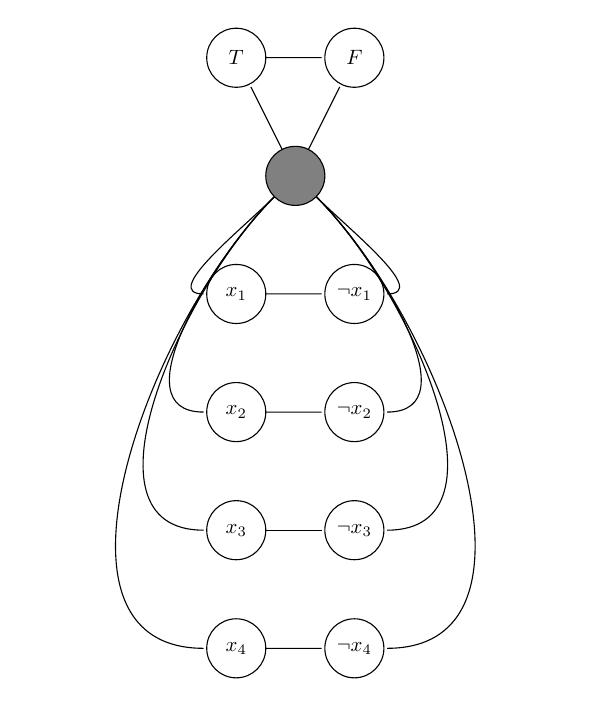
\begin{tikzpicture}[shorten >=1pt,node distance=2cm,auto,scale=1.5,nd/.style={draw=black,circle,scale=\sc,minimum width=0.75 cm,minimum height=1 cm},ndg/.style={nd,fill=gray}]
\def\sc{0.75}
\node[ndg] (R10) at (0.5,3) {};
\node[nd]  (R00) at (0,4)   {$T$};
\node[nd]  (R01) at (1,4)   {$F$};
\foreach \i in {1,...,4} {
  \node[nd]  (V\i0) at (0,3-\i)   {$x_{\i}$};
  \node[nd]  (V\i1) at (1,3-\i)   {$\neg x_{\i}$};
  \path (R10) edge[out=225,in=180] (V\i0);
  \path (R10) edge[out=315,in=0] (V\i1);
  \path (V\i0) edge (V\i1);
}
\foreach \i/\j in {10/00,00/01,10/01} {
  \path (R\i) edge (R\j);
}
\end{tikzpicture}